% 
% (c) Copyright 2016 Tabea Mendez
% 
% This source is free: you can redistribute it and/or modify
% it under the terms of the GNU General Public License as published by
% the Free Software Foundation, either version 3 of the License, or
% (at your option) any later version.
% 
% This source is distributed in the hope that it will be useful,
% but WITHOUT ANY WARRANTY; without even the implied warranty of
% MERCHANTABILITY or FITNESS FOR A PARTICULAR PURPOSE.  See the
% GNU General Public License for more details.
% 
% You should have received a copy of the GNU General Public License
% along with this source.  If not, see <http://www.gnu.org/licenses/>.
%
%%%%%%%%%%%%%%%%%%%%%%%%%%%%%%%%%%%%%%%%%%%%%%%%%%%%%%%%%%%%%%%%%%%%%%%%%%%%%%

\begin{description}
 \item [Definition:]$ $\\[0.2cm]
	\fcolorbox{CadetRed}{white}{$X(z) = \mysum{n=-\infty}{\infty}{x(n)\cdot z^{-n}}$}
 \item [Linearität:] Die z-Transformation ist linear.\\[0.2cm]
	\fcolorbox{CadetRed}{white}{$a_1\,x_1(n) + a_2\,x_2(n)\qquad\xrightarrow {\;\;\;Z\;\;\;}\qquad a_1\,X_1(z) + a_2\,X_2(z)$}
 \item [Verzögerung:] Verzögerung in der Zeit entsprich einer Multipikation mit $z^{-D}$ in der z-Transformation.\\[0.2cm]
	\fcolorbox{CadetRed}{white}{$x(n)\quad\xrightarrow {\;\;Z\;\;}\quad X(z)\qquad\Rightarrow \qquad x(n-D)\quad\xrightarrow {\;\;Z\;\;}\quad X(z)\cdot z^{-D}$}
 \item [Faltung:] Die Faltung in der Zeit entsprich der Multipikation in der z-Transformation\\[0.2cm]
	\fcolorbox{CadetRed}{white}{$y(n)=h(n)\ast x(n)\qquad\xrightarrow {\;\;\;Z\;\;\;}\qquad Y(z)=H(z)\cdot X(z)$}
\end{description}

\section{Konvergenzbereich (ROC)}
	Zum Konvergenzbereich (Region of Convergence) gehören alle komplexen z-Werte bei denen die z-Transformation einen endlichen Wert hat.\\[0cm]
	\textbf{Region of Convergence:}$\qquad$\fcolorbox{CadetRed}{white}{ROC $= \left\{z\in\mathbb{C}\;\left|\;X(z) = \mysum{n=-\infty}{\infty}{x(n)\cdot z^{-n}}\neq\pm \infty\right.\right\}$}\\[0.4cm]
	Zu einer z-Transformation muss \textbf{immer die ROC angegeben} werden. Ist keine ROC angegeben wird angenommen, dass das Zeitsignal kausal war. Hat eine z-Transformation keine ROC, so existiert diese nicht!\\[0.2cm]
	\fcolorbox{CadetRed}{white}{$\begin{array}{rcl}a^n\,u(n) \quad\xrightarrow{\;\; Z \;\;}\quad\dfrac{1}{1-a\,z^{-1}} && \text{ROC} = \left\{z\in\mathbb{C}\;\left|\;|z|>|a|\right.\right\}\\[0.5cm]-a^n\,u(-n-1) \quad\xrightarrow{\;\; Z \;\;}\quad\dfrac{1}{1-a\,z^{-1}} &\qquad\qquad& \text{ROC} = \left\{z\in\mathbb{C}\;\left|\;|z|<|a|\right.\right\}\end{array}$}$\quad$\fcolorbox{white}{white}{$\begin{array}{l}\rightarrow\quad\text{kausales Signal}\\[0.7cm]\rightarrow\quad\text{antikausales Signal}\end{array}$}\\[0.2cm]
	
	\begin{tikzpicture}[>=latex', scale=1.4]
		\def\s{3};
		\def\f{1.2};
		\def\r{0.8};

		\coordinate (c1) at (0,0);
		\draw[line width=0.75,fill=CadetRed, opacity=0.5](c1)++(-\s/2,-\s/2)--++(\s,0)--++(0,\s)--++(-\s,0)--cycle ;
		\draw[line width=0.75](c1)++(-\s/2,-\s/2)node[above right]{kausal}--++(\s,0)--++(0,\s)node[below left]{$z$-Plane}--++(-\s,0)--cycle node[below right, CadetRed]{\textbf{ROC}};

		\draw[line width=0.75,fill=white](c1)--++(-\f,0)--++(2*\f,0)--++(-\f,0)--++(0,-\f)--++(0,2*\f)--++(0,-\f)circle(\r);

		\draw[line width=0.75,fill](c1)++(-\f,0.7)circle(\r/30)node[above]{$z$};
		\draw[line width=0.75,->](c1)--node[rotate=-30, above right]{\footnotesize$|z|$}++(-\f,0.7);

		\draw[line width=0.75,fill](c1)++({\r*cos(30)},{\r*sin(30)})circle(\r/20)node[above right=-1pt,black]{$a$};%node[rotate=30,CadetRed]{\bm{$\times$}};
		\draw[line width=0.75,->](c1)--node[rotate=30, above ]{\footnotesize$|a|$}++({\r*cos(30)},{\r*sin(30)});


	\end{tikzpicture} $\qquad$
	\begin{tikzpicture}[>=latex', scale=1.4]
		\def\s{3};
		\def\f{1.2};
		\def\r{0.8};

		\coordinate (c1) at (0,0);
		\draw[line width=0.75,fill=white, opacity=0.5](c1)++(-\s/2,-\s/2)--++(\s,0)--++(0,\s)--++(-\s,0)--cycle ;
		\draw[line width=0.75](c1)++(-\s/2,-\s/2)node[above right]{antikausal}--++(\s,0)--++(0,\s)node[below left]{$z$-Plane}--++(-\s,0)--cycle node[below right, CadetRed]{\textbf{ROC}};

		\draw[line width=0.75,fill=CadetRed, opacity=0.5](c1)--++(-\f,0)--++(2*\f,0)--++(-\f,0)--++(0,-\f)--++(0,2*\f)--++(0,-\f)circle(\r);
		\draw[line width=0.75](c1)--++(-\f,0)--++(2*\f,0)--++(-\f,0)--++(0,-\f)--++(0,2*\f)--++(0,-\f)circle(\r);


		\draw[line width=0.75,fill](c1)++(-\f/2,0.2)circle(\r/30)node[above]{$z$};
		\draw[line width=0.75,->](c1)--node[rotate=-20, above]{\footnotesize$|z|$}++(-\f/2,0.2);

		\draw[line width=0.75,fill,black](c1)++({\r*cos(30)},{\r*sin(30)})circle(\r/20)node[above right=-1pt,black]{$a$};%node[rotate=30,CadetRed]{\bm{$\times$}};
		\draw[line width=0.75,->](c1)--node[rotate=30, above ]{\footnotesize$|a|$}++({\r*cos(30)},{\r*sin(30)});


	\end{tikzpicture}\\[0.cm]
	

\section{Kausalität und Stabilität}
	\begin{minipage}{0.5\textwidth}
		\textbf{Stabilitätsbedinung}\\[0.2cm]
		\fcolorbox{CadetRed}{white}{\parbox{6.5cm}{Der \textbf{Einheitskreis} der z-Ebene muss\\ \textbf{innerhalb} der ROC liegen!}}\\[0.3cm]
		\begin{tikzpicture}[>=latex', scale=1.1]
			\def\s{3};
			\def\f{1.3};
			\def\r{0.7};

			\coordinate (c1) at (0,0);
			\draw[line width=0.75](c1)++(-\s/2,-\s/2)node[above right]{ }--++(\s,0)--++(0,\s)node[below left]{$z$-Plane}--++(-\s,0)--cycle node[below right, CadetRed]{\textbf{ROC}};

			\draw[line width=0.75,fill=white](c1)--++(-\f,0)--++(2*\f,0)--++(-\f,0)--++(0,-\f)--++(0,2*\f);

			\draw[line width=1.5,dashed,CadetRed](c1)circle(0.9);
			\draw[line width=1.5,CadetRed](c1)++(0.9,0.1)--++(0,-0.2)node[below right=-1pt]{1};
		\end{tikzpicture}
	\end{minipage}
	\begin{minipage}{0.5\textwidth}
		\textbf{Grenzstabil}\\[0.2cm]
		\fcolorbox{CadetRed}{white}{\parbox{8.5cm}{Der Einheitskreis bildet die Grenze der der ROC$\quad\rightarrow\quad$ Pol liegt genau auf dem Einheitskreis!}}\\[0.3cm]
		\begin{tikzpicture}[>=latex', scale=1.1]
			\def\s{3};
			\def\f{1.3};
			\def\r{0.7};

			\coordinate (c1) at (0,0);
			\draw[line width=0.75](c1)++(-\s/2,-\s/2)node[above right]{ }--++(\s,0)--++(0,\s)node[below left]{$z$-Plane}--++(-\s,0)--cycle node[below right, CadetRed]{\textbf{ }};

			\draw[line width=0.75,fill=white](c1)--++(-\f,0)--++(2*\f,0)--++(-\f,0)--++(0,-\f)--++(0,2*\f);

			\draw[line width=1.5,dashed,CadetRed](c1)circle(0.9);
			\draw[line width=1.5,CadetRed](c1)++(0.9,0.1)--++(0,-0.2)node[below right=-1pt]{1};

			\draw[line width=0.75,fill,](c1)++(0.67,0.6)circle(\r/10)node[below left=0pt,black]{$p$};

		\end{tikzpicture}
	\end{minipage}
\newpage
	\subsection{Kausale Signale}
	\vspace*{-0.3cm}\begin{minipage}{0.43\textwidth}
		\textbf{Generelles kausales Signal: }\\[0.2cm]
		\fcolorbox{CadetRed}{white}{$\begin{array}{c}x(n) = A_1\,p_1^n\,u(n) + A_2\,p_2^n\,u(n) + ...\\[0.2cm]\text{\huge$\downarrow$}\;Z\\[0.1cm] X(z) = \dfrac{A_1}{1-p_1\,z^{-1}} + \dfrac{A_2}{1-p_2\,z^{-1}} + ...\end{array}$}\\[0.3cm]
	\end{minipage}
	\begin{minipage}{0.33\textwidth}
		\textbf{ROC: }$\,\,\;\;\;\quad$\\[0.2cm]\fcolorbox{CadetRed}{white}{ROC $= \left\{z\in\mathbb{C}\;\left|\;|z|>\max\limits_{i}^{}{|p_i|}\right.\right\}$}\\[0.2cm]
		\textbf{Stabilitätsbedinung:}$\qquad$\\[0.2cm]\fcolorbox{CadetRed}{white}{$\max\limits_{i}^{}{|p_i|}<1$}\\[-0.07cm]
	\end{minipage}
	\begin{minipage}{0.4\textwidth}
		\begin{tikzpicture}[>=latex', scale=1.4]
			\def\s{3};
			\def\f{1.3};
			\def\r{0.7};

			\coordinate (c1) at (0,0);
			\draw[line width=0.75,fill=CadetRed, opacity=0.5](c1)++(-\s/2,-\s/2)--++(\s,0)--++(0,\s)--++(-\s,0)--cycle ;
			\draw[line width=0.75](c1)++(-\s/2,-\s/2)node[above right]{kausal}--++(\s,0)--++(0,\s)node[below left]{$z$-Plane}--++(-\s,0)--cycle node[below right, CadetRed]{\textbf{ROC}};

			\draw[line width=0.75,fill=white](c1)--++(-\f,0)--++(2*\f,0)--++(-\f,0)--++(0,-\f)--++(0,2*\f)--++(0,-\f)circle(\r);

			\draw[line width=0.75,dashed](c1)--++(-\f,0)--++(2*\f,0)--++(-\f,0)--++(0,-\f)--++(0,2*\f)--++(0,-\f)circle(0.9);
			\draw[line width=0.75](c1)++(0.9,0.1)--++(0,-0.2)node[below right=-1pt]{1};

			\draw[line width=0.75,fill,](c1)++(0.35,0.6)circle(\r/15)node[below left=-2pt,black]{$p_4$};
			\draw[line width=0.75,fill,](c1)++(0.2,0)circle(\r/15)node[above right=-1pt,black]{$p_2$};
			\draw[line width=0.75,fill,](c1)++(0.35,-0.5)circle(\r/15)node[above left=-2pt,black]{$p_1$};
			\draw[line width=0.75,fill,](c1)++(-0.3,0.2)circle(\r/15)node[above=-1pt,black]{$p_3$};
		\end{tikzpicture}
	\end{minipage}\\[-0.3cm]

	\subsection{Antikausale Signale}
	\vspace*{-0.3cm}\begin{minipage}{0.43\textwidth}
		\textbf{Generelles antikausales Signal: }\\[0.2cm]
		\fcolorbox{CadetRed}{white}{$\begin{array}{c}x(n) = \text{-}B_1\,q_1^n\,u(\text{-}n\text{-}1) - B_2\,q_2^n\,u(\text{-}n\text{-}1) - ...\\[0.2cm]\text{\huge$\downarrow$}\;Z\\[0.1cm] X(z) = \dfrac{B_1}{1-q_1\,z^{-1}} + \dfrac{B_2}{1-q_2\,z^{-1}} + ...\end{array}$}\\[0.3cm]
	\end{minipage}
	\begin{minipage}{0.33\textwidth}
		\textbf{ROC: }$\,\,\;\;\;\quad$\\[0.2cm]\fcolorbox{CadetRed}{white}{ROC $= \left\{z\in\mathbb{C}\;\left|\;|z|<\min\limits_{i}^{}{|q_i|}\right.\right\}$}\\[0.2cm]
		\textbf{Stabilitätsbedinung:}$\qquad$\\[0.2cm]\fcolorbox{CadetRed}{white}{$\min\limits_{i}^{}{|q_i|}>1$}\\[-0.15cm]
	\end{minipage}
	\begin{minipage}{0.4\textwidth}
		\begin{tikzpicture}[>=latex', scale=1.4]
			\def\s{3};
			\def\f{1.3};
			\def\r{1.1};

			\coordinate (c1) at (0,0);
			\draw[line width=0.75,fill=white, opacity=0.5](c1)++(-\s/2,-\s/2)--++(\s,0)--++(0,\s)--++(-\s,0)--cycle ;
			\draw[line width=0.75](c1)++(-\s/2,-\s/2)node[above right]{kausal}--++(\s,0)--++(0,\s)node[below left]{$z$-Plane}--++(-\s,0)--cycle node[below right, CadetRed]{\textbf{ROC}};

			\draw[line width=0.75,fill=CadetRed, opacity=0.5](c1)--++(-\f,0)--++(2*\f,0)--++(-\f,0)--++(0,-\f)--++(0,2*\f)--++(0,-\f)circle(\r);
			\draw[line width=0.75](c1)--++(-\f,0)--++(2*\f,0)--++(-\f,0)--++(0,-\f)--++(0,2*\f)--++(0,-\f)circle(\r);


			\draw[line width=0.75,dashed](c1)--++(-\f,0)--++(2*\f,0)--++(-\f,0)--++(0,-\f)--++(0,2*\f)--++(0,-\f)circle(0.9);
			\draw[line width=0.75](c1)++(0.9,0.1)--++(0,-0.2)node[below left=-1pt,yshift=4pt]{1};
			\def\r{0.7};

			\draw[line width=0.75,fill,](c1)++(0.85,0.7)circle(\r/15)node[above right=-1pt,black]{$q_4$};
			\draw[line width=0.75,fill,](c1)++(1.3,0)circle(\r/15)node[above=-0pt,black]{$q_2$};
			\draw[line width=0.75,fill,](c1)++(0.8,-1.2)circle(\r/15)node[right=-0pt,black]{$q_1$};
			\draw[line width=0.75,fill,](c1)++(-1.3,0.4)circle(\r/15)node[above=-1pt,black]{$q_3$};
		\end{tikzpicture}
	\end{minipage}\\[-0.3cm]
	
	\subsection{Gemischte Signale}
	\begin{minipage}[t]{0.43\textwidth}
		\textbf{Generelles gemischtes Signal: }\\[0.2cm]
		\fcolorbox{CadetRed}{white}{$\begin{array}{c}x(n) = A_1\,p_1^n\,u(n) + A_2\,p_2^n\,u(n) + ...\text{\textcolor{white}{$xn\;\;\;\;$}}\\[0.2cm]\text{\textcolor{white}{$x(n)\;\,\;\;$}} \text{-}B_1\,q_1^n\,u(\text{-}n\text{-}1) - B_2\,q_2^n\,u(\text{-}n\text{-}1) - ...\\[0.2cm]\text{\huge$\downarrow$}\;Z\\[0.1cm] X(z) = \dfrac{A_1}{1-p_1\,z^{-1}} + \dfrac{A_2}{1-p_2\,z^{-1}} + ...\\[0.5cm] \text{\textcolor{white}{$X(z)$}} + \dfrac{B_1}{1-q_1\,z^{-1}} + \dfrac{B_2}{1-q_2\,z^{-1}} + ...\end{array}$}\\[0.3cm]
	\end{minipage}
	\begin{minipage}[t]{0.6\textwidth}
		\textbf{ROC: }$\,\,\;\;\;\quad$\\[0.275cm]\fcolorbox{CadetRed}{white}{ROC $= \left\{z\in\mathbb{C}\;\left|\;|z|>\max\limits_{i}^{}{|p_i|\quad\cap\quad|z|<\min\limits_{i}^{}{|q_i|}}\right.\right\}$}\\[0.2cm]
		\textbf{Stabilitätsbedinung:}$\qquad$\\[0.2cm]\fcolorbox{CadetRed}{white}{$\max\limits_{i}^{}{|p_i|}<1\quad\cap\quad\min\limits_{i}^{}{|q_i|}>1$}\\[-0.025cm]
	\end{minipage}\\[-3.2cm]
	\hspace*{14.05cm}\begin{minipage}{0.4\textwidth}
		\begin{tikzpicture}[>=latex', scale=1.4]
			\def\s{3};
			\def\f{1.3};
			\def\r{1.1};

			\coordinate (c1) at (0,0);
			\draw[line width=0.75,fill=white, opacity=0.5](c1)++(-\s/2,-\s/2)--++(\s,0)--++(0,\s)--++(-\s,0)--cycle ;
			\draw[line width=0.75](c1)++(-\s/2,-\s/2)node[above right]{kausal}--++(\s,0)--++(0,\s)node[below left]{$z$-Plane}--++(-\s,0)--cycle node[below right, CadetRed]{\textbf{ROC}};

			\draw[line width=0.75,fill=CadetRed, opacity=0.5](c1)--++(-\f,0)--++(2*\f,0)--++(-\f,0)--++(0,-\f)--++(0,2*\f)--++(0,-\f)circle(\r);
			\draw[line width=0.75](c1)--++(-\f,0)--++(2*\f,0)--++(-\f,0)--++(0,-\f)--++(0,2*\f)--++(0,-\f)circle(\r);

			\def\r{0.7};
			\draw[line width=0.75,fill=white](c1)--++(-\f,0)--++(2*\f,0)--++(-\f,0)--++(0,-\f)--++(0,2*\f)--++(0,-\f)circle(\r);

			\draw[line width=0.75,dashed](c1)--++(-\f,0)--++(2*\f,0)--++(-\f,0)--++(0,-\f)--++(0,2*\f)--++(0,-\f)circle(0.9);
			\draw[line width=0.75](c1)++(0.9,0.1)--++(0,-0.2)node[below right=-3pt,yshift=2pt]{1};

			\draw[line width=0.75,fill,](c1)++(0.85,0.7)circle(\r/15)node[above right=-1pt,black]{$q_2$};
			\draw[line width=0.75,fill,](c1)++(-1.3,0.4)circle(\r/15)node[above=-1pt,black]{$q_1$};

			\draw[line width=0.75,fill,](c1)++(0.2,0)circle(\r/15)node[above right=-1pt,black]{$p_2$};
			\draw[line width=0.75,fill,](c1)++(0.41,-0.56)circle(\r/15)node[above left=-2pt,black]{$p_1$};
		\end{tikzpicture}
	\end{minipage}\\[-0.8cm]

	
\section{Inverse z-Transformation}
	Um eine z-Transformation, die als \textbf{gebrochen rationale Funktion} dargestellt werden kann, in die Zeit zurückzutransformieren sind folgende Schritte notwendig:
	\begin{itemize}
	 \item Die z-Transformation in Partialbrüche der Form $\dfrac{1}{1-a\,z^{-1}}$ zerlegen
	 \item Jeden Partialbruch mit Hilfe folgender Beziehung und dem Wissen, ob der Pol kausal oder anitkausal ist, zurückzutransformieren.\\[0.2cm]
	\fcolorbox{white}{white}{$\begin{array}{lr}\text{kausales Signal}&\quad\rightarrow\\[0.7cm]\text{antikausales Signal}&\quad\rightarrow\end{array}$}$\quad$\fcolorbox{CadetRed}{white}{$\begin{array}{rcl}a^n\,u(n) \quad\xrightarrow{\;\; Z \;\;}\quad\dfrac{1}{1-a\,z^{-1}} && \text{ROC} = \left\{z\in\mathbb{C}\;\left|\;|z|>|a|\right.\right\}\\[0.5cm]-a^n\,u(-n-1) \quad\xrightarrow{\;\; Z \;\;}\quad\dfrac{1}{1-a\,z^{-1}} &\qquad\qquad& \text{ROC} = \left\{z\in\mathbb{C}\;\left|\;|z|<|a|\right.\right\}\end{array}$}
	\item Bei Doppelpolen folgende Rücktransformationen verwenden.\\[0.2cm]
	\fcolorbox{white}{white}{$\begin{array}{lr}\text{kausales Signal}&\rightarrow\\[0.7cm]\text{antikausales Signal}&\rightarrow\end{array}$}\fcolorbox{CadetRed}{white}{$\begin{array}{rcl}(n+1)\,a^n\,u(n) \quad\xrightarrow{\;\; Z \;\;}\quad\dfrac{1}{(1-a\,z^{-1})^2} && \text{ROC} = \left\{z\in\mathbb{C}\;\left|\;|z|>|a|\right.\right\}\\[0.5cm]-(n+1)\,a^n\,u(-n-1) \quad\xrightarrow{\;\; Z \;\;}\quad\dfrac{1}{(1-a\,z^{-1})^2} &\qquad& \text{ROC} = \left\{z\in\mathbb{C}\;\left|\;|z|<|a|\right.\right\}\end{array}$}
	 \item Konstanten werden zu gewichteten Diracs zurücktransformiert.$\qquad$ \fcolorbox{CadetRed}{white}{$ A_0 \delta(n) \xrightarrow{\;\;Z\;\;} A_0$}
	\end{itemize}
	
	\subsection{Partialbruchzerlegung bei einfachen Polen}
		Bei der Partialbruchzerlegung einer gebrochen rationalen Funktion werden drei Fälle unterschieden:\\[0.3cm]
		\begin{minipage}{0.4\textwidth}
			\begin{itemize}
			\item $M > N\quad$ echt gebrochen\\[-0.35cm]
			\item $M = N\quad$ unecht gebrochen\\[-0.35cm]
			\item $M < N\quad$ unecht gebrochen\\[-0.35cm]
			\end{itemize}
		\end{minipage}
		\begin{minipage}{0.3\textwidth}
			\fcolorbox{CadetRed}{white}{$X(z) = \dfrac{N(z)}{D(z)} = \dfrac{b_0 + b_1\,z^{-1} + b_2\,z^{-2} + \dots + b_N\,z^{-N} }{1 + a_1\,z^{-1} + a_2\,z^{-2} + \dots + a_M\,z^{-M} }$}
		\end{minipage}

		\begin{tabularx}{\textwidth}{|p{1.6cm}|X|}
		 \hline&\\[-0.3cm]
			\bm{$M > N$}
			& $X(z) = \dfrac{N(z)}{D(z)} = \dfrac{N(z)}{(1 - p_1\,z^{-1})\,\dots\,(1 - p_M\,z^{-1}) } = \dfrac{A_1}{(1 - p_1\,z^{-1})} + \dots + \dfrac{A_M}{(1 - p_M\,z^{-1})}$\\[0.6cm]
			&\fcolorbox{CadetRed}{white}{$A_i = \left[(1 - p_i\,z^{-1})\cdot X(z)\right]_{z=p_i} = \left[\dfrac{N(z)}{\myprod{j\neq i}{}{(1 - p_j\,z^{-1})}}\right]_{z=p_i}$}\\[1cm]
		 \hline&\\[-0.3cm]
			\bm{$M = N$} & $X(z) = \dfrac{N(z)}{D(z)} = \dfrac{N(z)}{(1 - p_1\,z^{-1})\,\dots\,(1 - p_M\,z^{-1}) } = A_0 + \dfrac{A_1}{(1 - p_1\,z^{-1})} + \dots + \dfrac{A_M}{(1 - p_M\,z^{-1})}$\\[0.6cm]
			&\fcolorbox{CadetRed}{white}{$A_0 = X(z)|_{z=0} $}$\quad\qquad$\fcolorbox{CadetRed}{white}{$A_i$ siehe Fall $M>N$}\\[0.3cm]
		 \hline&\\[-0.3cm]
			\bm{$M < N$} & $X(z) = \dfrac{N(z)}{D(z)}\;\overset{\text{Polynom-}}{\underset{\text{division}}{=}} \; Q(z) + \dfrac{R(z)}{D(z)}$\\[0.6cm]
			& $Q(z) = B_0 + B_1\,z^{-1} + ... + B_{N-M}\,z^{-(N-M)}\quad\xrightarrow{\;\; Z^{-1}\;\;}\quad B_0\,\delta(n) + \,\delta(n\text{-}1) + ... + B_{N-M}\,\delta(n\text{-}(N\text{-}M))$\\[0.4cm]
			& $\dfrac{R(z)}{D(z)} = \dfrac{R(z)}{(1 - p_1\,z^{-1})\,\dots\,(1 - p_M\,z^{-1}) } = \dfrac{A_1}{(1 - p_1\,z^{-1})} + \dots + \dfrac{A_M}{(1 - p_M\,z^{-1})}$\\[0.6cm]
			&\fcolorbox{CadetRed}{white}{$A_i$ siehe Fall $M>N$}\\[0.3cm]
		 \cline{2-2}&\\[-0.3cm]
			& $X(z) = \dfrac{N(z)}{D(z)} = N(z)\cdot W(z) $\\[0.4cm]
			& \fcolorbox{CadetRed}{white}{Nur $W(z)$ wie im Fall $M>N$ zurücktransformierten$\quad\Rightarrow\quad w(n)$}\\[0.4cm]
			& $W(z) = \dfrac{1}{D(z)} = \dfrac{1}{(1 - p_1\,z^{-1})\,\dots\,(1 - p_M\,z^{-1}) } = \dfrac{A_1}{(1 - p_1\,z^{-1})} + \dots + \dfrac{A_M}{(1 - p_M\,z^{-1})}$\\[0.5cm]
			&\fcolorbox{CadetRed}{white}{$A_i$ siehe Fall $M>N$}\\[0.4cm]
			& $X(z) = N(z)\cdot W(z) = b_0\cdot W(z) + b_1\,z^{-1}\cdot W(z) + b_2\,z^{-2}\cdot W(z) + \dots + b_N\,z^{-N}\cdot W(z)$\\[0.4cm]
			& \fcolorbox{CadetRed}{white}{$x(n)$ ist die Summe der mit $b_i$ gewichteten und um $i$ verzögerten $w(n)$}\\[0.3cm]
		 \hline
		\end{tabularx}

\newpage
\section{Frequenzspektrum}
	Das Frequenzspektrum (DTFT) eines diskreten Signals $x(n)$ und ist definiert als:\\[0.2cm]
	\fcolorbox{CadetRed}{white}{$X(\omega) = \mysum{n=-\infty}{\infty}{x(n)\,\e^{-j\omega n}}$}$\qquad$ und die inverse DTFT als:$\qquad$\fcolorbox{CadetRed}{white}{$x(n) = \dfrac{1}{2\pi}\,\myint{-\pi}{\pi}{X(\omega)\,\e^{j\omega n}}{\omega}$}\\[0.2cm]

	\subsection{Vergleich zwischen analogem Signal \bm{$x(nT)$} und digitalen Signal \bm{$x(n)$}}
		\begin{tabularx}{\textwidth}{|p{3cm}|X|X|}
		\hline&&\\[-0.35cm]
			&\textbf{Analoges Signal \bm{$x(nT)$}} & \textbf{Diskretes Signal \bm{$x(n)$}}\\[0.05cm]
		\hline&&\\[-0.35cm]
			\textbf{DTFT}& $\hat X(f)=\mysum{n=-\infty}{\infty}{x(nT)\cdot \e^{-j2\pi fTn}}$ &$X(\omega) = \mysum{n=-\infty}{\infty}{x(n)\,\e^{-j\omega n}}$\\[0.35cm]
		\hline&&\\[-0.35cm]
			\textbf{Periode}& $f_s$  & $2\,\pi$ \\[0.05cm]
		\hline&&\\[-0.35cm]
			\textbf{inverse DTFT}&$x(nT)=\dfrac{1}{f_s}\,\myint{-f_s/2}{f_2/2}{\hat X(f)\cdot \e^{j2\pi fTn}}{f}$ &$x(n) = \dfrac{1}{2\pi}\,\myint{-\pi}{\pi}{X(\omega)\,\e^{j\omega n}}{\omega}$\\[0.45cm]
		\hline
		\end{tabularx}\\
	
	\subsection{Geometrische Interpretation des Frequenzganges}
		\begin{minipage}{0.44\textwidth}
			Der Frequenzgang $X(\omega)$ entspricht der Übertragungsfunktion $X(z)$ auf dem Einheitskreis:\\[0.3cm]
			\fcolorbox{CadetRed}{white}{$z=\e^{j\omega}$}$\qquad\Rightarrow\qquad$\fcolorbox{CadetRed}{white}{$X(\omega) = X(z)|_{z=\e^{j\omega}}$}\\[0.3cm]
			Damit der Frequenzgang existiert, muss der Einheitskreis \textbf{innerhalb der Region of Convergence (ROC)} liegen.
		\end{minipage}\begin{minipage}{0.03\textwidth}$ $\end{minipage}
		\begin{minipage}{0.27\textwidth}
			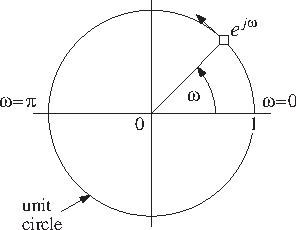
\includegraphics[width = 1\textwidth]{pic/geoFrequenzgang.pdf}\\
		\end{minipage}
		\begin{minipage}{0.26\textwidth}
			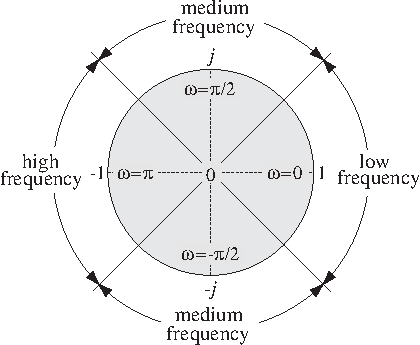
\includegraphics[width = 1\textwidth]{pic/frequency.pdf}
		\end{minipage}
		\begin{itemize}
			 \item Wenn $\omega$ von $-\pi$ bis $\pi$ variert, wendert $z$ auf dem Einheitskreis von $-1$ über $0$ nach $-1$.
			 \item Die tiefen Frequenzen sind bei $z \approx 1 $ und die hohen bei $z \approx -1 $. Bei $z \approx \pm j$ sind die mittleren Frequenzen.
		\end{itemize}$ $\\[-0.1cm]
		\begin{minipage}{0.7\textwidth}
			Anhand der Pol- und Nullstellen in der z-Ebene,\\ kann der Frequenzgang $|X(\omega)|$ skizziert werden.\\[0.3cm]
			\fcolorbox{CadetRed}{white}{$|X(\omega_0)| = \dfrac{\myprod{i}{\text{\textcolor{white}{a}}}{\text{Abstand von }\e^{j\omega_0}\text{ zur Nullstelle }z_i}}{\myprod{j}{\text{\textcolor{white}{a}}}{\text{Abstand von }\e^{j\omega_0}\text{ zum Pol }p_j}}$}\\[0.3cm]
			Daraus lassen sich folgende Grundsätze ableiten\\[-0.3cm]
			\begin{itemize}
				\item Je näher der Punkt auf dem Einheitskreis einer Nullstelle kommt,\\ desto kleiner wird der Frequenzgang.\\[-0.25cm]
				\item Je näher der Punkt auf dem Einheitskreis einem Pol kommt, desto\\ grösser wird der Frequenzgang.\\[-0.25cm]
				\item Sitzt der Pol genau auf dem Einheitskreis, so wird der Frequenzgang\\ an dieser stelle unendlich gross.
			\end{itemize}
		\end{minipage}
		\hspace*{-4cm}\begin{minipage}{0.5\textwidth}
			\vspace*{-0.5cm}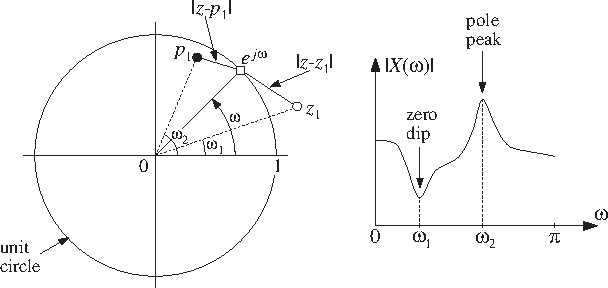
\includegraphics[width = 1\textwidth]{pic/geoFrequenzgangPN.pdf}\\
			\hspace*{3.5cm}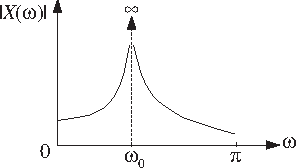
\includegraphics[width = 0.6\textwidth]{pic/polAufEinheitskreis.pdf}
		\end{minipage}$ $\\

	\subsection{Fourierpärchen}
		\vspace*{-0.2cm}\begin{minipage}{0.68\textwidth}
			\begin{tabular}{l|c|c}
				& $x(n)$ & $X(\omega)$ (Nyquistintervall)\\[0.1cm]
			\hline&&\\[-0.3cm]
				\text{Komplexe Schwingung} $\quad$& $\e^{j\omega_0 n}$ & $2\pi\,\delta(\omega-\omega_0)$\\[0.2cm]
				\text{Cosinusschwingung} & $\cos(\omega_0 n)$ & $\pi\,\delta(\omega-\omega_0) + \pi\,\delta(\omega+\omega_0)$\\[0.2cm]
				\text{Sinusschwingung} & $\sin(\omega_0 n)$ & $-j\pi\,\delta(\omega-\omega_0) + j\pi\,\delta(\omega+\omega_0)$\\[0.1cm]
			\hline
			\end{tabular}
		\end{minipage}
		\begin{minipage}{0.3\textwidth}
			\textbf{Satz des Parseval:}\\[0.2cm]\fcolorbox{CadetRed}{white}{$E = \mysum{n=-\infty}{\infty}{|x(n)|^2} = \dfrac{1}{2\pi}\,\myint{-\pi}{\pi}{|H(\omega)|^2}{\omega}$}\\
		\end{minipage}
	
	


